\begin{figure}
\centering
\tikzset{every picture/.style={line width=0.75pt}} %set default line width to 0.75pt          

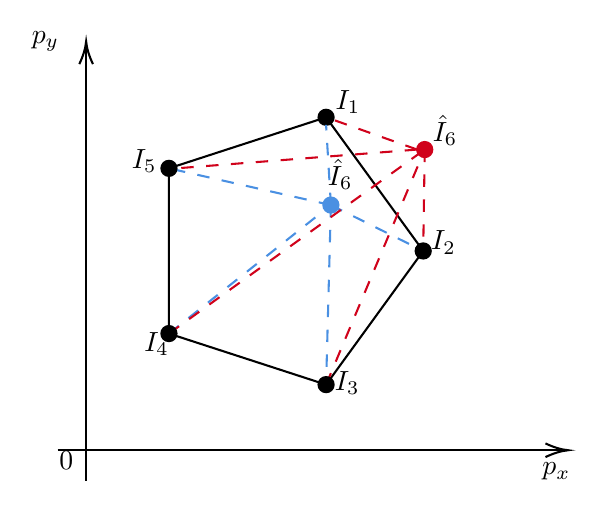
\begin{tikzpicture}[x=0.75pt,y=0.75pt,yscale=-1,xscale=1]
%uncomment if require: \path (0,847); %set diagram left start at 0, and has height of 847

%Shape: Polygon [id:dp224164202141931] 
\draw   (366.92,228.47) -- (320.13,292.88) -- (244.42,268.28) -- (244.42,188.67) -- (320.13,164.07) -- cycle ;
%Shape: Ellipse [id:dp3256341156223599] 
\draw  [color={rgb, 255:red, 208; green, 2; blue, 27 }  ,draw opacity=1 ][fill={rgb, 255:red, 208; green, 2; blue, 27 }  ,fill opacity=1 ] (364.01,179.62) .. controls (364.01,177.61) and (365.65,175.98) .. (367.66,175.98) .. controls (369.67,175.98) and (371.3,177.61) .. (371.3,179.62) .. controls (371.3,181.63) and (369.67,183.26) .. (367.66,183.26) .. controls (365.65,183.26) and (364.01,181.63) .. (364.01,179.62) -- cycle ;
%Straight Lines [id:da8764490533518536] 
\draw [color={rgb, 255:red, 74; green, 144; blue, 226 }  ,draw opacity=1 ][line width=0.75]  [dash pattern={on 4.5pt off 4.5pt}]  (322.45,206.36) -- (366.92,228.47) ;
%Straight Lines [id:da6851668490079947] 
\draw [color={rgb, 255:red, 74; green, 144; blue, 226 }  ,draw opacity=1 ][line width=0.75]  [dash pattern={on 4.5pt off 4.5pt}]  (322.45,206.36) -- (320.13,292.88) ;
%Straight Lines [id:da23609417084914575] 
\draw [color={rgb, 255:red, 74; green, 144; blue, 226 }  ,draw opacity=1 ][line width=0.75]  [dash pattern={on 4.5pt off 4.5pt}]  (244.42,268.28) -- (322.45,206.36) ;
%Straight Lines [id:da2571972397860731] 
\draw [color={rgb, 255:red, 74; green, 144; blue, 226 }  ,draw opacity=1 ][line width=0.75]  [dash pattern={on 4.5pt off 4.5pt}]  (322.45,206.36) -- (244.42,188.67) ;
%Straight Lines [id:da2251639682861042] 
\draw [color={rgb, 255:red, 208; green, 2; blue, 27 }  ,draw opacity=1 ][line width=0.75]  [dash pattern={on 4.5pt off 4.5pt}]  (320.13,292.88) -- (367.66,179.62) ;
%Straight Lines [id:da7789718802550452] 
\draw [color={rgb, 255:red, 208; green, 2; blue, 27 }  ,draw opacity=1 ][line width=0.75]  [dash pattern={on 4.5pt off 4.5pt}]  (244.42,268.28) -- (367.66,179.62) ;
%Straight Lines [id:da23249730714159367] 
\draw [color={rgb, 255:red, 208; green, 2; blue, 27 }  ,draw opacity=1 ][line width=0.75]  [dash pattern={on 4.5pt off 4.5pt}]  (367.66,179.62) -- (366.92,228.47) ;
%Straight Lines [id:da6827372695149887] 
\draw [color={rgb, 255:red, 208; green, 2; blue, 27 }  ,draw opacity=1 ][line width=0.75]  [dash pattern={on 4.5pt off 4.5pt}]  (364.01,179.62) -- (320.13,164.07) ;
%Shape: Ellipse [id:dp7050237810455391] 
\draw  [fill={rgb, 255:red, 0; green, 0; blue, 0 }  ,fill opacity=1 ] (363.28,228.47) .. controls (363.28,226.46) and (364.91,224.83) .. (366.92,224.83) .. controls (368.93,224.83) and (370.56,226.46) .. (370.56,228.47) .. controls (370.56,230.49) and (368.93,232.12) .. (366.92,232.12) .. controls (364.91,232.12) and (363.28,230.49) .. (363.28,228.47) -- cycle ;
%Shape: Ellipse [id:dp9309501596310132] 
\draw  [fill={rgb, 255:red, 0; green, 0; blue, 0 }  ,fill opacity=1 ] (316.49,164.07) .. controls (316.49,162.06) and (318.12,160.43) .. (320.13,160.43) .. controls (322.14,160.43) and (323.77,162.06) .. (323.77,164.07) .. controls (323.77,166.09) and (322.14,167.72) .. (320.13,167.72) .. controls (318.12,167.72) and (316.49,166.09) .. (316.49,164.07) -- cycle ;
%Shape: Ellipse [id:dp7614343877717125] 
\draw  [fill={rgb, 255:red, 0; green, 0; blue, 0 }  ,fill opacity=1 ] (240.78,188.67) .. controls (240.78,186.66) and (242.41,185.03) .. (244.42,185.03) .. controls (246.43,185.03) and (248.07,186.66) .. (248.07,188.67) .. controls (248.07,190.68) and (246.43,192.32) .. (244.42,192.32) .. controls (242.41,192.32) and (240.78,190.68) .. (240.78,188.67) -- cycle ;
%Shape: Ellipse [id:dp936113035140345] 
\draw  [fill={rgb, 255:red, 0; green, 0; blue, 0 }  ,fill opacity=1 ] (240.78,268.28) .. controls (240.78,266.26) and (242.41,264.63) .. (244.42,264.63) .. controls (246.43,264.63) and (248.07,266.26) .. (248.07,268.28) .. controls (248.07,270.29) and (246.43,271.92) .. (244.42,271.92) .. controls (242.41,271.92) and (240.78,270.29) .. (240.78,268.28) -- cycle ;
%Shape: Ellipse [id:dp14199884674981345] 
\draw  [fill={rgb, 255:red, 0; green, 0; blue, 0 }  ,fill opacity=1 ] (316.49,292.88) .. controls (316.49,290.86) and (318.12,289.23) .. (320.13,289.23) .. controls (322.14,289.23) and (323.77,290.86) .. (323.77,292.88) .. controls (323.77,294.89) and (322.14,296.52) .. (320.13,296.52) .. controls (318.12,296.52) and (316.49,294.89) .. (316.49,292.88) -- cycle ;
%Shape: Ellipse [id:dp35213262674036416] 
\draw  [color={rgb, 255:red, 74; green, 144; blue, 226 }  ,draw opacity=1 ][fill={rgb, 255:red, 74; green, 144; blue, 226 }  ,fill opacity=1 ] (318.8,206.36) .. controls (318.8,204.35) and (320.43,202.72) .. (322.45,202.72) .. controls (324.46,202.72) and (326.09,204.35) .. (326.09,206.36) .. controls (326.09,208.38) and (324.46,210.01) .. (322.45,210.01) .. controls (320.43,210.01) and (318.8,208.38) .. (318.8,206.36) -- cycle ;
%Straight Lines [id:da36974497752955027] 
\draw [line width=0.75]    (190.8,324.49) -- (434.77,324.49) ;
\draw [shift={(436.77,324.49)}, rotate = 180] [color={rgb, 255:red, 0; green, 0; blue, 0 }  ][line width=0.75]    (10.93,-3.29) .. controls (6.95,-1.4) and (3.31,-0.3) .. (0,0) .. controls (3.31,0.3) and (6.95,1.4) .. (10.93,3.29)   ;
%Straight Lines [id:da37889403281928824] 
\draw [line width=0.75]    (204.52,339.19) -- (204.52,129.52) ;
\draw [shift={(204.52,127.52)}, rotate = 90] [color={rgb, 255:red, 0; green, 0; blue, 0 }  ][line width=0.75]    (10.93,-3.29) .. controls (6.95,-1.4) and (3.31,-0.3) .. (0,0) .. controls (3.31,0.3) and (6.95,1.4) .. (10.93,3.29)   ;
%Straight Lines [id:da8075828784484049] 
\draw [color={rgb, 255:red, 208; green, 2; blue, 27 }  ,draw opacity=1 ][line width=0.75]  [dash pattern={on 4.5pt off 4.5pt}]  (364.01,179.62) -- (248.07,188.67) ;
%Straight Lines [id:da06190541080915435] 
\draw [color={rgb, 255:red, 74; green, 144; blue, 226 }  ,draw opacity=1 ][line width=0.75]  [dash pattern={on 4.5pt off 4.5pt}]  (322.45,206.36) -- (320.13,167.72) ;

% Text Node
\draw (323.23,149.49) node [anchor=north west][inner sep=0.75pt]  [font=\normalsize]  {$I_{1}$};
% Text Node
\draw (369.25,217.36) node [anchor=north west][inner sep=0.75pt]  [font=\normalsize]  {$I_{2}$};
% Text Node
\draw (322.86,285.22) node [anchor=north west][inner sep=0.75pt]  [font=\normalsize]  {$I_{3}$};
% Text Node
\draw (231.06,266.42) node [anchor=north west][inner sep=0.75pt]  [font=\normalsize]  {$I_{4}$};
% Text Node
\draw (225.1,177.92) node [anchor=north west][inner sep=0.75pt]  [font=\normalsize]  {$I_{5}$};
% Text Node
\draw (319.55,182.82) node [anchor=north west][inner sep=0.75pt]  [font=\normalsize]  {$\hat{I}_{6}$};
% Text Node
\draw (370.06,161.75) node [anchor=north west][inner sep=0.75pt]  [font=\normalsize]  {$\hat{I}_{6}$};
% Text Node
\draw (422.83,329.15) node [anchor=north west][inner sep=0.75pt]    {$p_{x}$};
% Text Node
\draw (176.86,121.4) node [anchor=north west][inner sep=0.75pt]    {$p_{y}$};
% Text Node
\draw (190.14,323.58) node [anchor=north west][inner sep=0.75pt]    {$0$};


\end{tikzpicture}
\caption{Illustration of interpolation vs. extrapolation. Consider $\KK=\{1,2,3,4,5,6\}$ and $\KU=\{x,y\}$. Note that $q_x$ and $q_y$ are latent variables to $\KK$, influencing the observed interference at each link of $\KK$. The positions of $I_1,I_2\ldots I_5$ are affected by the value of $q_x$ and $q_y$ at the moment of observation. Estimations are performed for the link $6$, denoted by $\hat{I}_6$ with blue and red dots. The blue is from intertropolation, as it falls in-between the known observations (i.e. the convex hull), whereas the red is from extrapolation. }
\label{fig: constrained_lr}
\end{figure}